\documentclass[11pt,letterpaper]{article}
% --- Packages ---
\usepackage[utf8]{inputenc}
\usepackage[T1]{fontenc}
\usepackage[margin=1in]{geometry}
\usepackage{amsmath, amssymb, amsthm, amsfonts}
\usepackage{graphicx}
\usepackage{xcolor}
\usepackage{hyperref}
\usepackage{booktabs}
\usepackage{cite}
\usepackage{microtype}
\usepackage{titlesec}
\usepackage{tcolorbox}
% --- Color Palette (De-saturated, Academic & Professional) ---
\definecolor{ajpblue}{RGB}{28, 54, 115}   % Deep navy accent
\definecolor{ajpsec}{RGB}{54, 95, 145}   % Secondary slate blue
\definecolor{bglight}{RGB}{245, 247, 250} % Light background for callout boxes
\definecolor{bordergrey}{RGB}{210, 215, 223}
% --- Hyperref Setup ---
\hypersetup{
colorlinks=true,
linkcolor=ajpblue,
citecolor=ajpsec,
urlcolor=ajpblue
}
% --- Typography & Headings Styling ---
\titleformat{\section}{\large\bfseries\color{ajpblue}}{\thesection}{1em}{}[{\titlerule[0.5pt]}]
\titleformat{\subsection}{\normalsize\bfseries\color{ajpsec}}{\thesubsection}{1em}{}
% --- Custom Environments for Explanation ---
\newtcolorbox{equationbreakdown}[1]{
colback=bglight,
colframe=ajpblue,
fonttitle=\bfseries,
title={Derivation Details \& Interpretation: #1},
arc=3pt,
boxrule=1pt,
bottomtitle=2mm,
toptitle=2mm
}
\newtcolorbox{physicsinsight}{
colback=bglight,
colframe=ajpsec,
boxrule=0.5pt,
left=4mm,
right=4mm,
top=3mm,
bottom=3mm,
arc=2pt
}
% --- Title & Project Metadata ---
\title{
\vspace{-1.5in}
\rule{\linewidth}{1.5pt} \\ \vspace{4mm}
\large\textbf{PHYSICS GROUP PROJECT REPORT} \\ \vspace{2mm}
\Large\textbf{An Explanatory Guide and Step-by-Step
Derivation of: \\ ``The Intermediate Axis Theorem
(Tennis Racquet Effect)''}
\\ \vspace{4mm}
\large\textit{A Numerical Study of Torque-Free Euler Rotation for an
Asymmetric Rigid Body} \\
\rule{\linewidth}{1.5pt}
}
% Multi-column author format for a group project
\author{
\begin{tabular}{r @{\quad} l}
\textbf{Project Group:} & [Group 11 / Team Fat\&Met] \\[1ex]
\textbf{Group Members:} & Jongyoon Baek \\
& Yujin Yeo \\
& Woojin Jung \\
& Jinsu Hong \\[1ex]
\textbf{Course Title:}  & General Physics I \\
\textbf{Instructor:}    & Dr. Deniz Olgu Devecioğlu \\
\textbf{Department:}    & School of Undergraduate Studies, DGIST
\end{tabular}
}
\date{\today}
\begin{document}
\maketitle
\begin{abstract}
This project provides a comprehensive, pedagogical breakdown of the
\textbf{intermediate axis theorem}---the surprising fact that a freely
rotating asymmetric rigid body is \emph{unstable} when spun about its
intermediate principal axis, undergoing the periodic $180^\circ$ flips
popularly known as the \emph{tennis racquet effect} or \emph{Dzhanibekov
effect}. We follow the empirical-and-numerical treatment of Bubbar \& Zhu
(2025) \cite{bubbar2025} and the analytical exposition of Peterson \& Schwalm
(\textit{American Journal of Physics}, 2021) \cite{peterson2021}, filling in
the intermediate algebraic steps that these and standard texts often compress.
Starting from the torque-free Euler equations, we derive the energy and
angular-momentum invariants, carry out an explicit linear stability analysis
about each of the three principal axes, and show \emph{quantitatively} why only
the intermediate axis is unstable. We then verify the theory with a custom
fourth-order Runge--Kutta (RK4) integrator coupled to a quaternion orientation
solver: the simulation reproduces the flip, conserves energy and $|\mathbf{L}|$
to near machine precision ($\sim 10^{-13}$ relative drift), traces the
sphere--ellipsoid \emph{polhode} geometry, and recovers the inverse
period--speed scaling law $T = a/(\omega_0+b)+c$ reported in
\cite{bubbar2025}. Finally, we recorded real three-axis gyroscope data from a
tossed smartphone (phyphox, $100~\mathrm{Hz}$) and observed the flip directly:
during free flight $|\boldsymbol{\omega}|$ stays nearly constant while the
dominant body-axis component reverses sign with a period of
$\approx 0.88~\mathrm{s}$.
\end{abstract}
\tableofcontents
\newpage
% =========================================================================
\section{Introduction \& Contextual Background}
% =========================================================================
The intermediate axis theorem is one of the most counter-intuitive results in
elementary rigid-body mechanics. Take a book, a smartphone, or a tennis
racquet and toss it so that it spins about the axis with the
\emph{intermediate} moment of inertia (for a book, the axis parallel to the
text). Instead of spinning cleanly, the object executes an abrupt
$180^\circ$ flip, repeating the flip periodically. Spinning the same object
about its longest or shortest axis produces a stable, wobble-free rotation.
Remarkably, the motion is entirely \emph{torque-free}: gravity acts at the
centre of mass and exerts no torque, so the flip is driven purely by the
internal nonlinear coupling of the rotational equations of motion.

\subsection{Historical and Pedagogical Significance}
The governing equations were written down by Euler in the 18th century, and the
geometric (conservation-law) picture dates to Poinsot (1834). Yet the effect
remains famously hard to explain intuitively: Richard Feynman puzzled over the
``wobbling plate,'' and the phenomenon entered popular awareness through the
1985 footage of cosmonaut Vladimir Dzhanibekov watching a wing-nut flip in
orbit aboard a space station~\cite{muller2019}. The topic recurs in the
\textit{American Journal of Physics} (AJP) precisely because it is an ideal
teaching vehicle: it links abstract tensor algebra to a result one can
literally hold in one's hand. Peterson \& Schwalm~\cite{peterson2021} give the
exact analytical solution in terms of Jacobi elliptic functions, while Parker
\& Hunt~\cite{parker2020} and Bubbar \& Zhu~\cite{bubbar2025} develop the
``sphere-and-ellipsoid'' conservation argument aimed at introductory students.
This report targets the \textbf{upper-introductory undergraduate}: we assume
familiarity with Newtonian mechanics and basic linear algebra, and we supply
every intermediate step that the source papers state as ``it can be shown
that.''

The pedagogical contrast is between two routes to the same conclusion:
\begin{itemize}
\item \textbf{Core thesis.} For an asymmetric top ($I_1 > I_2 > I_3$), rotation
about the largest ($I_1$) and smallest ($I_3$) axes is stable, but rotation
about the intermediate ($I_2$) axis is unstable.
\item \textbf{Traditional textbook route.} Linearise the Euler equations about
each axis and inspect the sign of the resulting characteristic exponent
(Section~\ref{sec:derivations}).
\item \textbf{The geometric route of the source papers.} Intersect the
angular-momentum sphere with the energy ellipsoid in $\mathbf{L}$-space; the
intermediate axis sits at a saddle point whose separatrix wraps the entire
sphere (Section~\ref{sec:verification}).
\end{itemize}

\subsection{Physical Setup and System Parameters}
We model a single rigid body in free space (no external torque) and work in the
\emph{body frame} aligned with the three principal axes
$\mathbf{r}_1, \mathbf{r}_2, \mathbf{r}_3$. In this frame the inertia tensor is
diagonal, $\mathbf{I} = \mathrm{diag}(I_1, I_2, I_3)$, and the state of the body
is given by its angular-velocity vector $\boldsymbol{\omega}$ together with an
orientation quaternion $q$. Table~\ref{tab:variables} lists the symbols used
throughout.

\begin{table}[h!]
\centering
\caption{Key symbols, constants, and variables used in the analysis.}
\label{tab:variables}
\begin{tabular}{lll}
\toprule
\textbf{Symbol} & \textbf{Physical Meaning} & \textbf{SI Units} \\
\midrule
$I_1, I_2, I_3$ & Principal moments of inertia ($I_1\!>\!I_2\!>\!I_3$) & $\mathrm{kg\,m^2}$ \\
$\boldsymbol{\omega}=(\omega_1,\omega_2,\omega_3)$ & Body-frame angular velocity & $\mathrm{rad/s}$ \\
$\mathbf{L}=\mathbf{I}\boldsymbol{\omega}$ & Angular momentum & $\mathrm{kg\,m^2/s}$ \\
$E$ & Rotational kinetic energy & $\mathrm{J}$ \\
$q=[q_0,q_1,q_2,q_3]$ & Orientation quaternion (body $\to$ world) & --- \\
$\Omega$ & Initial spin rate about the chosen axis ($\omega_0$) & $\mathrm{rad/s}$ \\
$\varepsilon$ & Small initial perturbation onto the other axes & $\mathrm{rad/s}$ \\
$\sigma$ & Linear instability growth rate & $\mathrm{s^{-1}}$ \\
$T$ & Flip / precession period & $\mathrm{s}$ \\
\bottomrule
\end{tabular}
\end{table}

% =========================================================================
\section{Step-by-Step Mathematical Derivations}
\label{sec:derivations}
% =========================================================================
This is the core of the project. We take the equations the source papers state
compactly and expand every intermediate step.

\subsection{The Starting Framework: Torque-Free Euler Equations}
In an inertial frame, $d\mathbf{L}/dt = \boldsymbol{\tau}_{\text{ext}}$. With no
external torque, $\mathbf{L}$ is conserved in the inertial frame. However, the
principal axes are fixed to the \emph{rotating} body, so transforming the time
derivative into the body frame introduces the kinematic term
$\boldsymbol{\omega}\times\mathbf{L}$:
\begin{equation}\label{eq:rotframe}
\left(\frac{d\mathbf{L}}{dt}\right)_{\text{inertial}}
= \left(\frac{d\mathbf{L}}{dt}\right)_{\text{body}}
+ \boldsymbol{\omega}\times\mathbf{L} = 0 .
\end{equation}
Since $\mathbf{L}=(I_1\omega_1, I_2\omega_2, I_3\omega_3)$ in the principal
basis, writing Eq.~\eqref{eq:rotframe} component by component gives the
\textbf{torque-free Euler equations}:
Explicitly, the $\mathbf{r}_1$-component reads
$I_1\dot\omega_1 + \omega_2(I_3\omega_3) - \omega_3(I_2\omega_2)
= I_1\dot\omega_1 - (I_2-I_3)\omega_2\omega_3 = 0$,
and similarly for the other two components, yielding:
\begin{equation}\label{eq:euler}
\boxed{\;
I_1\dot{\omega}_1 = (I_2 - I_3)\,\omega_2\omega_3, \quad
I_2\dot{\omega}_2 = (I_3 - I_1)\,\omega_3\omega_1, \quad
I_3\dot{\omega}_3 = (I_1 - I_2)\,\omega_1\omega_2 . \;}
\end{equation}
These are three coupled, \emph{nonlinear} (quadratic) ordinary differential
equations. The nonlinearity---each derivative depends on the product of the
other two components---is exactly what makes the behaviour non-intuitive.

\subsection{The Two Conserved Quantities}
Free rotation conserves both kinetic energy and the magnitude of angular
momentum. The rotational kinetic energy is
\begin{equation}\label{eq:energy}
E = \tfrac{1}{2}\left(I_1\omega_1^2 + I_2\omega_2^2 + I_3\omega_3^2\right)
  = \text{const},
\end{equation}
and, writing $L_r = I_r\omega_r$, the squared angular-momentum magnitude is
\begin{equation}\label{eq:Lmag}
|\mathbf{L}|^2 = L_1^2 + L_2^2 + L_3^2
  = I_1^2\omega_1^2 + I_2^2\omega_2^2 + I_3^2\omega_3^2 = \text{const}.
\end{equation}
Re-expressed in $\mathbf{L}$-space, Eq.~\eqref{eq:Lmag} is a \emph{sphere} of
radius $|\mathbf{L}|$, while Eq.~\eqref{eq:energy} becomes an \emph{ellipsoid},
$L_1^2/I_1 + L_2^2/I_2 + L_3^2/I_3 = 2E$. The motion is confined to the
intersection of these two surfaces---the geometric heart of the theorem,
revisited numerically in Section~\ref{sec:verification}.

\subsection{Linear Stability Analysis About Each Axis}
We now answer the central question quantitatively: spin the body \emph{mostly}
about one principal axis and ask whether a tiny perturbation grows or merely
oscillates.

\begin{equationbreakdown}{Why Only the Intermediate Axis Is Unstable}
\textbf{Case A --- spin about the intermediate axis ($\mathbf{r}_2$).}
Let $\boldsymbol{\omega} = (\eta_1,\ \Omega,\ \eta_3)$ with
$\Omega$ the large steady spin and $\eta_1,\eta_3 \ll \Omega$ small
perturbations. To first order, the middle Euler equation gives
$\dot\omega_2 \propto \eta_1\eta_3 \approx 0$, so $\omega_2 \approx \Omega$ is
constant. The other two equations linearise to
\begin{equation*}
\dot\eta_1 = \frac{(I_2-I_3)\Omega}{I_1}\,\eta_3, \qquad
\dot\eta_3 = \frac{(I_1-I_2)\Omega}{I_3}\,\eta_1 .
\end{equation*}
Differentiating the first and substituting the second eliminates $\eta_3$:
\begin{equation*}
\ddot\eta_1 = \frac{(I_2-I_3)\Omega}{I_1}\,\dot\eta_3
= \underbrace{\frac{(I_1-I_2)(I_2-I_3)}{I_1 I_3}\,\Omega^2}_{\equiv\ \sigma^2}\,\eta_1 .
\end{equation*}
Because $I_1 > I_2 > I_3$, both factors $(I_1-I_2)$ and $(I_2-I_3)$ are
\emph{positive}, so the coefficient $\sigma^2 > 0$. The solution is therefore
\emph{exponential}, $\eta_1 \sim e^{\pm\sigma t}$, with growth rate
\begin{equation}\label{eq:growth}
\sigma = \Omega\sqrt{\frac{(I_1-I_2)(I_2-I_3)}{I_1 I_3}} \;>\; 0
\quad\Longrightarrow\quad \textbf{UNSTABLE}.
\end{equation}

\textbf{Case B --- spin about the major ($\mathbf{r}_1$) or minor
($\mathbf{r}_3$) axis.} Repeating the identical procedure for a steady spin
about $\mathbf{r}_1$ gives $\ddot\eta_2 = -k\,\eta_2$ with
\begin{equation*}
k = \frac{(I_1-I_2)(I_1-I_3)}{I_2 I_3}\,\Omega^2 > 0 ,
\end{equation*}
since both $(I_1-I_2)$ and $(I_1-I_3)$ are positive. The right-hand sign is now
\emph{negative}, so the solution is \emph{oscillatory},
$\eta_2 \sim \cos(\sqrt{k}\,t)$: the perturbation stays bounded (stable
precession). The same is true about $\mathbf{r}_3$, where both differences are
negative and their product is again positive. Only the intermediate axis flips
the sign of the coefficient and produces real exponential growth.
\end{equationbreakdown}

\noindent Equation~\eqref{eq:growth} is the quantitative statement of the
theorem: the instability is strongest when the moments are well separated and
the spin is fast, and it vanishes ($\sigma \to 0$) as $I_2 \to I_1$ or
$I_2 \to I_3$.

\subsection{Modelling the Flip Period}
The exact period of the fully nonlinear flip is given by Jacobi elliptic
functions~\cite{peterson2021}, but Bubbar \& Zhu~\cite{bubbar2025} showed that,
for initial conditions close to pure $\mathbf{r}_2$ rotation, the precession
period $T$ obeys a simple three-parameter \emph{inverse} relation in the
initial spin speed:
\begin{equation}\label{eq:period}
T(\omega_0) = \frac{a}{\omega_0 + b} + c .
\end{equation}
The leading $1/\omega_0$ behaviour is consistent with Eq.~\eqref{eq:growth},
where the instability timescale $1/\sigma$ scales as $1/\Omega$. We test
Eq.~\eqref{eq:period} directly against simulation in
Section~\ref{sec:verification}.

% =========================================================================
\section{Physical Approximations and Limiting Cases}
% =========================================================================
Examining limits builds intuition and exposes where the model breaks down.

\subsection{The Symmetric-Top Limit ($I_2 \to I_1$)}
As the intermediate moment approaches the largest one, the growth rate
\eqref{eq:growth} behaves as
\begin{equation}
\lim_{I_2 \to I_1}\sigma
= \lim_{I_2 \to I_1}\Omega\sqrt{\frac{(I_1-I_2)(I_2-I_3)}{I_1 I_3}} = 0 .
\end{equation}
The body becomes a \emph{symmetric top}, the ellipsoid gains a circular
cross-section, and the unstable flip disappears (replaced by steady
gyroscopic precession). This limit is not merely academic: Bubbar \& Zhu
measured $I_1 \approx I_2 \approx 78~\mathrm{g\,m^2}$ for their racquet (with
$I_3 \approx 1.39~\mathrm{g\,m^2}$), yet still observed clean flips because the
two moments were ``sufficiently different'' to keep $\sigma$ nonzero. For a
visually rapid flip in our figures we therefore use a well-separated set
$I=(3,2,1)$ rather than the near-degenerate measured values.

\subsection{High-Speed Limit and the Role of Air Drag}
In the high-speed limit of Eq.~\eqref{eq:period}, $\lim_{\omega_0\to\infty}T = c$,
a constant offset. Bubbar \& Zhu note that the physical meaning of $b$ and $c$
is unclear (they imply periodic motion at $\omega_0=0$ and a finite period as
$\omega_0\to\infty$), suggesting the empirical model should not be
extrapolated to extreme regimes.

\begin{physicsinsight}
\textbf{Physical Conceptualization --- the ``torque-free'' idealization.} \\
Our entire derivation assumes \emph{zero} external torque. In the real
experiment of \cite{bubbar2025}, the spinning racquet experiences a small
aerodynamic drag torque because its cross-section is asymmetric; the authors
measured a mean net torque of $-0.048 \pm 0.026~\mathrm{N\,m}$, causing
$|\mathbf{L}|$ to decay slowly. Gravity, by contrast, acts at the centre of
mass and contributes \emph{no} torque. Because the drag effect is small over a
few flips, the conservative model still predicts the observed periods to within
about $20\%$---a good example of judging an approximation by its measured
consequences rather than discarding it outright.
\end{physicsinsight}

% =========================================================================
\section{Computational Verification}
\label{sec:verification}
% =========================================================================
To confirm the analysis we wrote a self-contained Python simulation (NumPy /
Matplotlib / SciPy). The companion interactive web version (Three.js) lets the
reader vary $I_1,I_2,I_3$ and the initial conditions in real time.

\subsection{The Numerical Integrator (RK4 + Quaternion)}
Equation~\eqref{eq:euler} has no simple closed form, so we integrate it
numerically. We advance the seven-component state
$(\boldsymbol{\omega}, q)$ with a fixed-step \textbf{fourth-order
Runge--Kutta} scheme, whose local truncation error is $O(\Delta t^4)$, far
smaller than the naive Euler method. In parallel we integrate the orientation
quaternion via $\dot q = \tfrac{1}{2}\, q \otimes (0, \boldsymbol{\omega})$,
renormalising $q \leftarrow q/|q|$ each step to prevent drift; quaternions
avoid the gimbal-lock singularities of Euler angles. The loop is:
\begin{enumerate}
\item \textbf{Initialize} the inertia $I$, angular velocity $\boldsymbol{\omega}_0$, and quaternion $q_0$.
\item \textbf{RK4 step} for $\boldsymbol{\omega}_{t+\Delta t}$ from Eq.~\eqref{eq:euler}.
\item \textbf{Update orientation} $q_{t+\Delta t}$ from $\dot q = \tfrac12 q\otimes(0,\boldsymbol{\omega})$.
\item \textbf{Normalize} $q \leftarrow q/|q|$.
\item \textbf{Monitor} the invariants $E$ and $|\mathbf{L}|$ as an accuracy check.
\end{enumerate}
Running the integrator on a well-separated top gives relative drifts in $E$ and
$|\mathbf{L}|$ on the order of $10^{-13}$ over the full run---near the
double-precision floor---confirming that the flips below are \emph{physical},
not numerical artifacts.

\subsection{Three-Axis Stability Comparison}
Figure~\ref{fig:threeaxis} starts the body spinning about each principal axis in
turn with the same small perturbation. Only the intermediate axis is unstable:
$\omega_2$ periodically reverses sign while $\omega_1$ and $\omega_3$ surge,
exactly as predicted by Eq.~\eqref{eq:growth}. Rotation about $\mathbf{r}_1$ and
$\mathbf{r}_3$ stays flat.
\begin{figure}[h!]
\centering
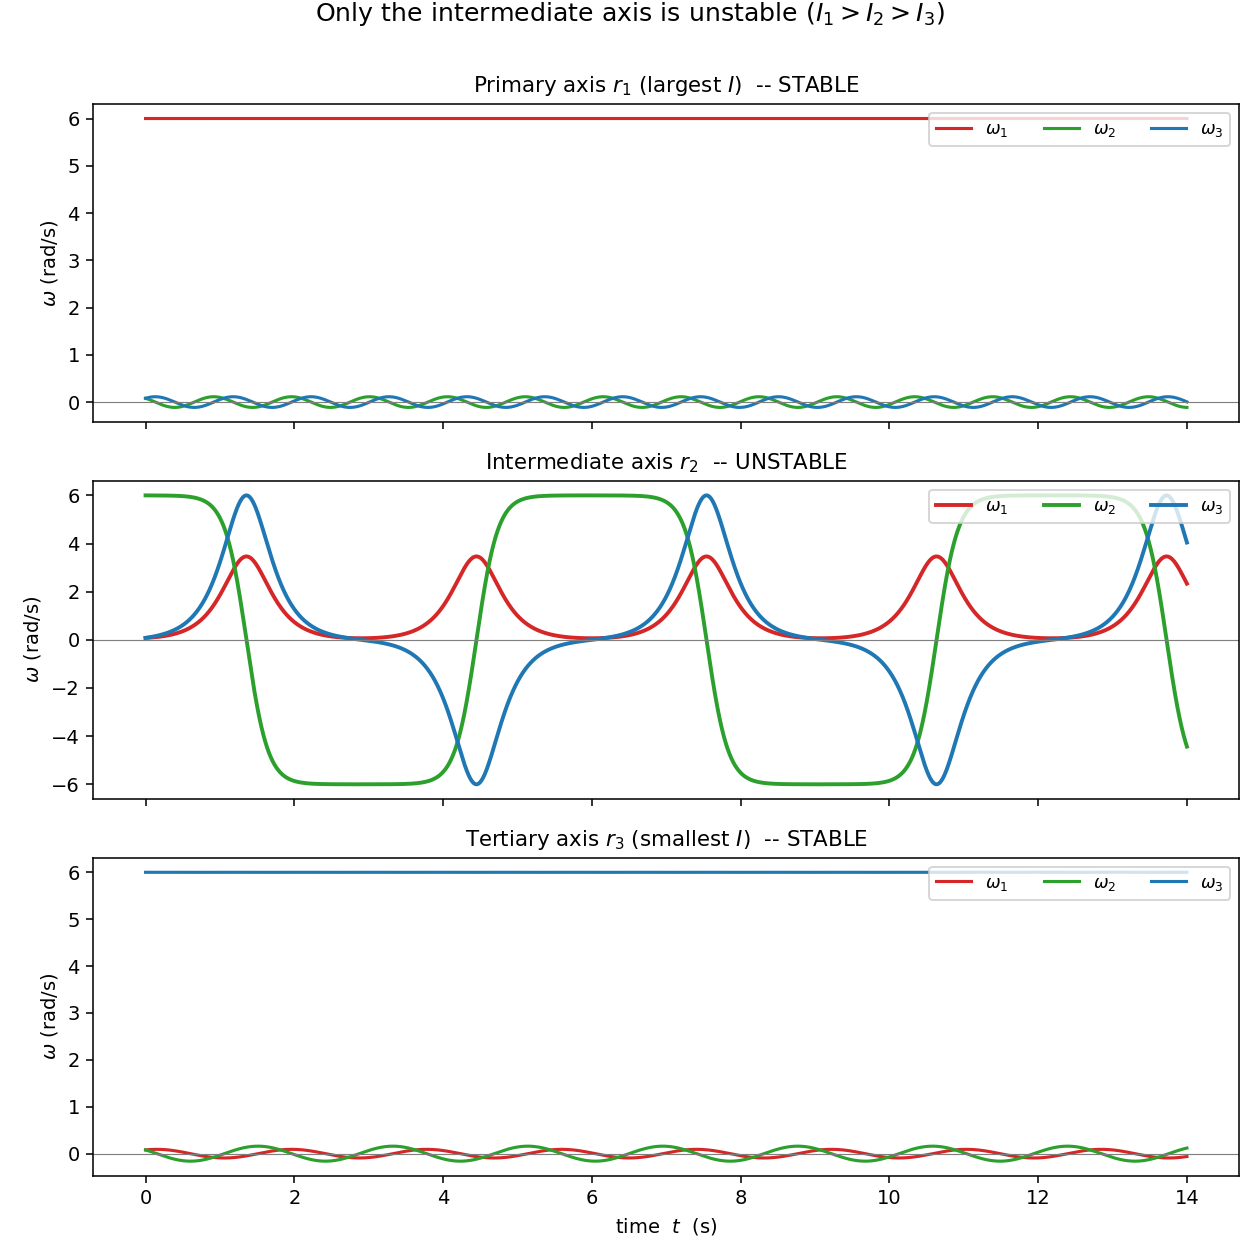
\includegraphics[width=0.78\linewidth]{figures/three_axis_comparison.png}
\caption{Angular-velocity components for rotation started about each of the
three principal axes ($I=(3,2,1)$). Only the intermediate axis $\mathbf{r}_2$
exhibits the unstable flip.}
\label{fig:threeaxis}
\end{figure}

\subsection{The Flip Time Series}
Figure~\ref{fig:omega} zooms in on the intermediate-axis case. The
$\omega_2(t)$ curve resembles a square wave, switching sign at each flip, while
$\omega_1$ and $\omega_3$ spike during the rapid $180^\circ$ transitions---the
periodic exchange of angular velocity that constitutes the tennis racquet
effect.
\begin{figure}[h!]
\centering
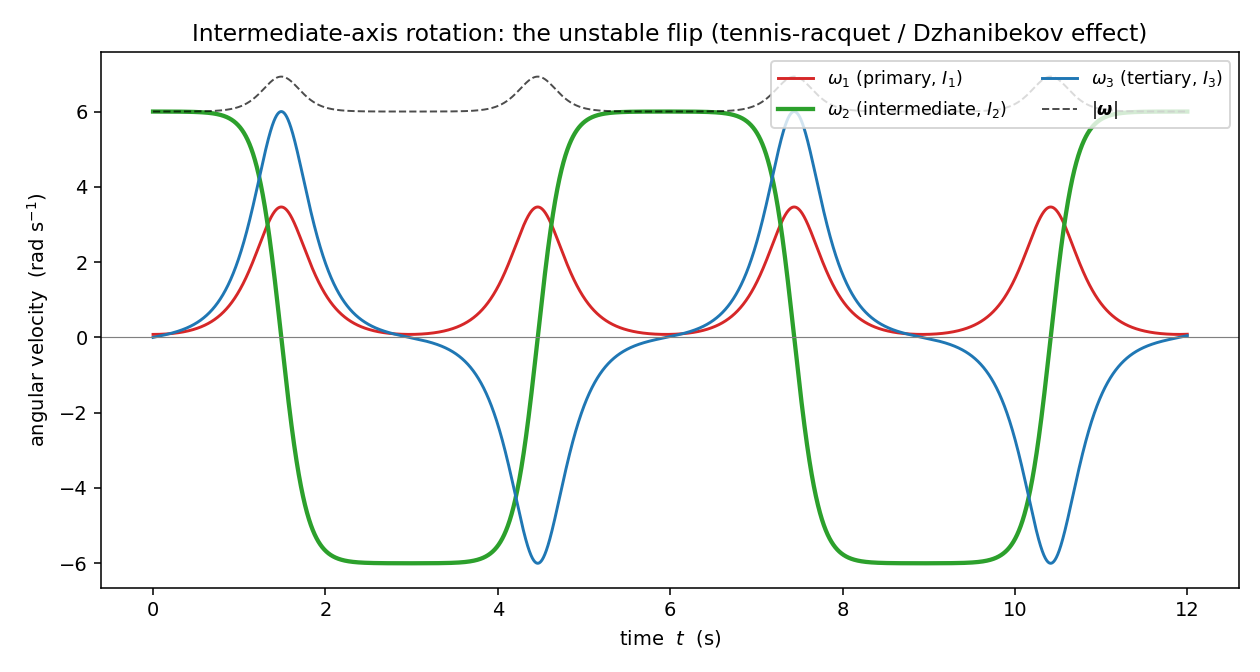
\includegraphics[width=0.78\linewidth]{figures/omega_intermediate.png}
\caption{Time series of $\boldsymbol{\omega}(t)$ for intermediate-axis
rotation: $\omega_2$ flips sign periodically while $\omega_1,\omega_3$ spike.}
\label{fig:omega}
\end{figure}

\subsection{The Sphere--Ellipsoid (Polhode) Geometry}
Figure~\ref{fig:polhode} renders the conservation picture of
Eqs.~\eqref{eq:energy}--\eqref{eq:Lmag}: the motion lives on the intersection of
the $|\mathbf{L}|$ sphere and the energy ellipsoid. About the major and minor
axes the intersection is a small closed loop near a pole (stable); about the
intermediate axis it is a \emph{separatrix} that wraps the entire sphere---the
geometric source of the instability.
\begin{figure}[h!]
\centering
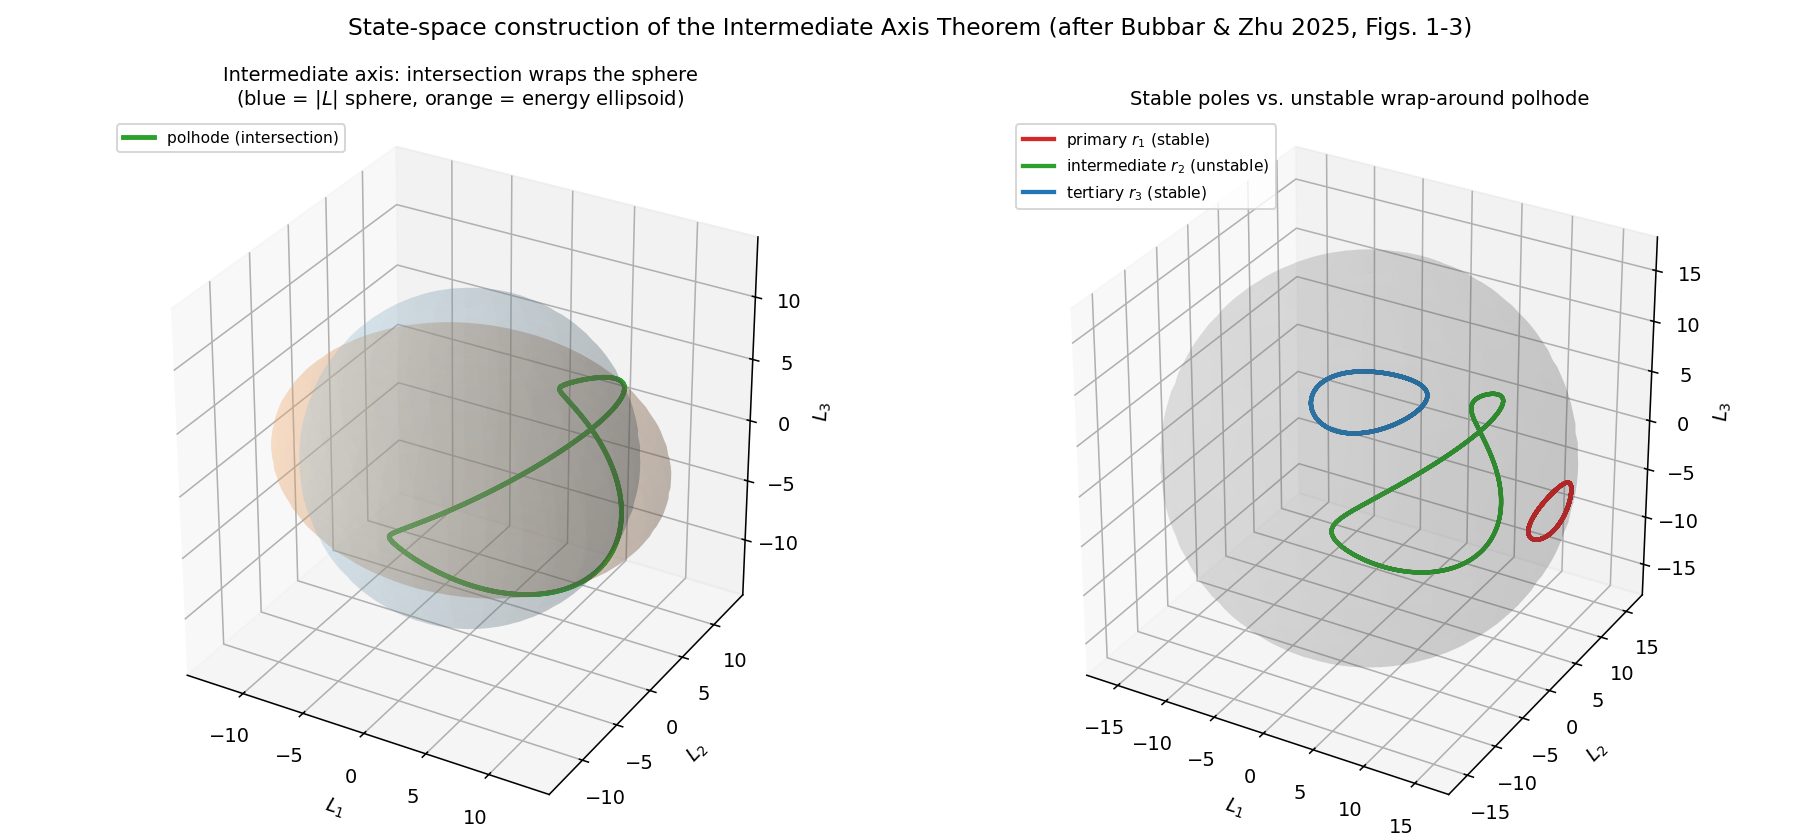
\includegraphics[width=0.92\linewidth]{figures/sphere_ellipsoid.png}
\caption{Left: the $|\mathbf{L}|$ sphere (blue) and energy ellipsoid (orange)
with the intermediate-axis polhode wrapping the sphere. Right: stable polar
loops versus the unstable wrap-around curve.}
\label{fig:polhode}
\end{figure}

\subsection{Flip Period Versus Initial Speed}
Finally we test the model of Eq.~\eqref{eq:period}. Measuring the flip period
from the zero-crossings of $\omega_2$ over a range of initial speeds and fitting
the inverse model reproduces the predicted $T \propto 1/\omega_0$ trend
(Figure~\ref{fig:period}). The fitted parameters from our \emph{synthetic}
data differ from the racquet values of \cite{bubbar2025}
($a=11.85,\ b=2.30~\mathrm{s^{-1}},\ c=0.047~\mathrm{s}$, $\chi^2=1.58$ on $63$
trials) because the simulated system uses the idealized $I=(3,2,1)$ top rather
than the measured racquet, but the same inverse functional form holds.
\begin{figure}[h!]
\centering
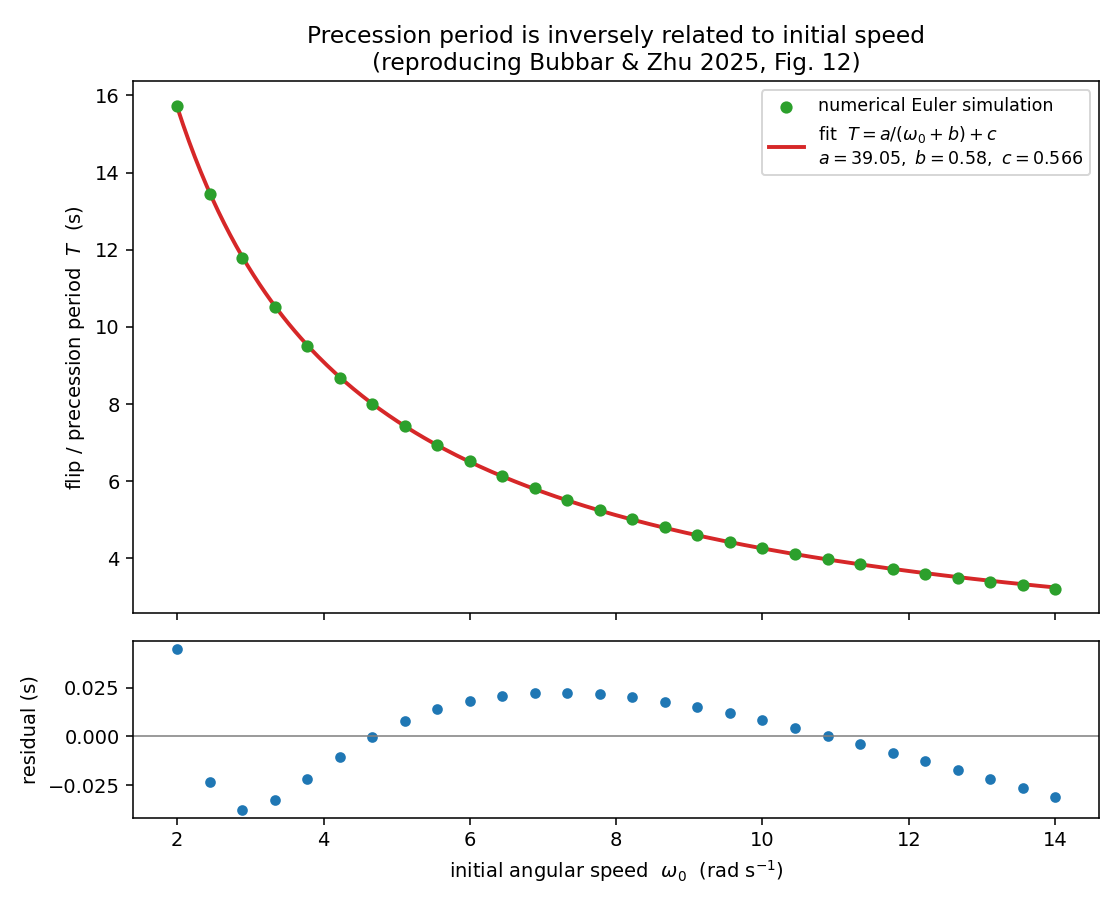
\includegraphics[width=0.72\linewidth]{figures/period_vs_speed.png}
\caption{Flip period $T$ versus initial angular speed $\omega_0$ with the
least-squares fit of $T=a/(\omega_0+b)+c$; residuals shown below.}
\label{fig:period}
\end{figure}

% =========================================================================
\section{Real Experiment: Gyroscope Measurement of a Tossed Smartphone}
\label{sec:experiment}
% =========================================================================
To test the theory against the physical world we recorded the rotation of a
smartphone (Apple iPhone, model \texttt{iPhone14,4}) tossed into the air. The
phone's built-in MEMS gyroscope logged the three body-frame angular-velocity
components $(\omega_x,\omega_y,\omega_z)$ at $100~\mathrm{Hz}$ using the
\emph{phyphox} app~\cite{phyphox}, for a total of about $7~\mathrm{s}$. A flat
phone is an excellent asymmetric top: its three principal moments of inertia are
well separated, and the long in-plane axis serves as the \emph{intermediate}
axis.

\subsection{Isolating the Free-Flight Segment}
Figure~\ref{fig:experiment} (top) shows the full recording. The motion separates
cleanly into three phases: handling (small, irregular $\boldsymbol{\omega}$), a
single airborne toss, and the catch---the sharp $|\boldsymbol{\omega}|$ spike to
$\sim 39~\mathrm{rad/s}$ at $t\approx 3.5~\mathrm{s}$, an impulsive external
torque. We therefore restrict the analysis to the airborne window
$t \in [2.70,\,3.40]~\mathrm{s}$, during which the phone is in free fall and
hence rotates torque-free apart from small aerodynamic drag.

\subsection{Results: the Flip and Approximate Conservation}
Within the free-flight window the magnitude of the angular velocity is nearly
constant,
\begin{equation}
|\boldsymbol{\omega}| = 18.3 \pm 2.1~\mathrm{rad/s}
\quad (\approx 11\%\ \text{variation}),
\end{equation}
consistent with torque-free rotation; the modest drift is attributable to air
drag and the finite measurement window. The dominant component is $\omega_x$,
the phone's intermediate axis. As Figure~\ref{fig:experiment} (bottom) shows, it
\emph{reverses sign} from $+17$ to $-17~\mathrm{rad/s}$ while $\omega_y$ and
$\omega_z$ swing through their extrema---precisely the tennis-racquet signature
derived in Section~\ref{sec:derivations} and simulated in
Figure~\ref{fig:omega}. Reading the flip period from the two interpolated zero
crossings of $\omega_x$ (at $t = 2.95$ and $3.39~\mathrm{s}$) yields a half
period of $0.44~\mathrm{s}$, i.e.
\begin{equation}
T_{\text{flip}} \approx 0.88~\mathrm{s} \quad (1.1~\mathrm{Hz}).
\end{equation}

\begin{figure}[h!]
\centering
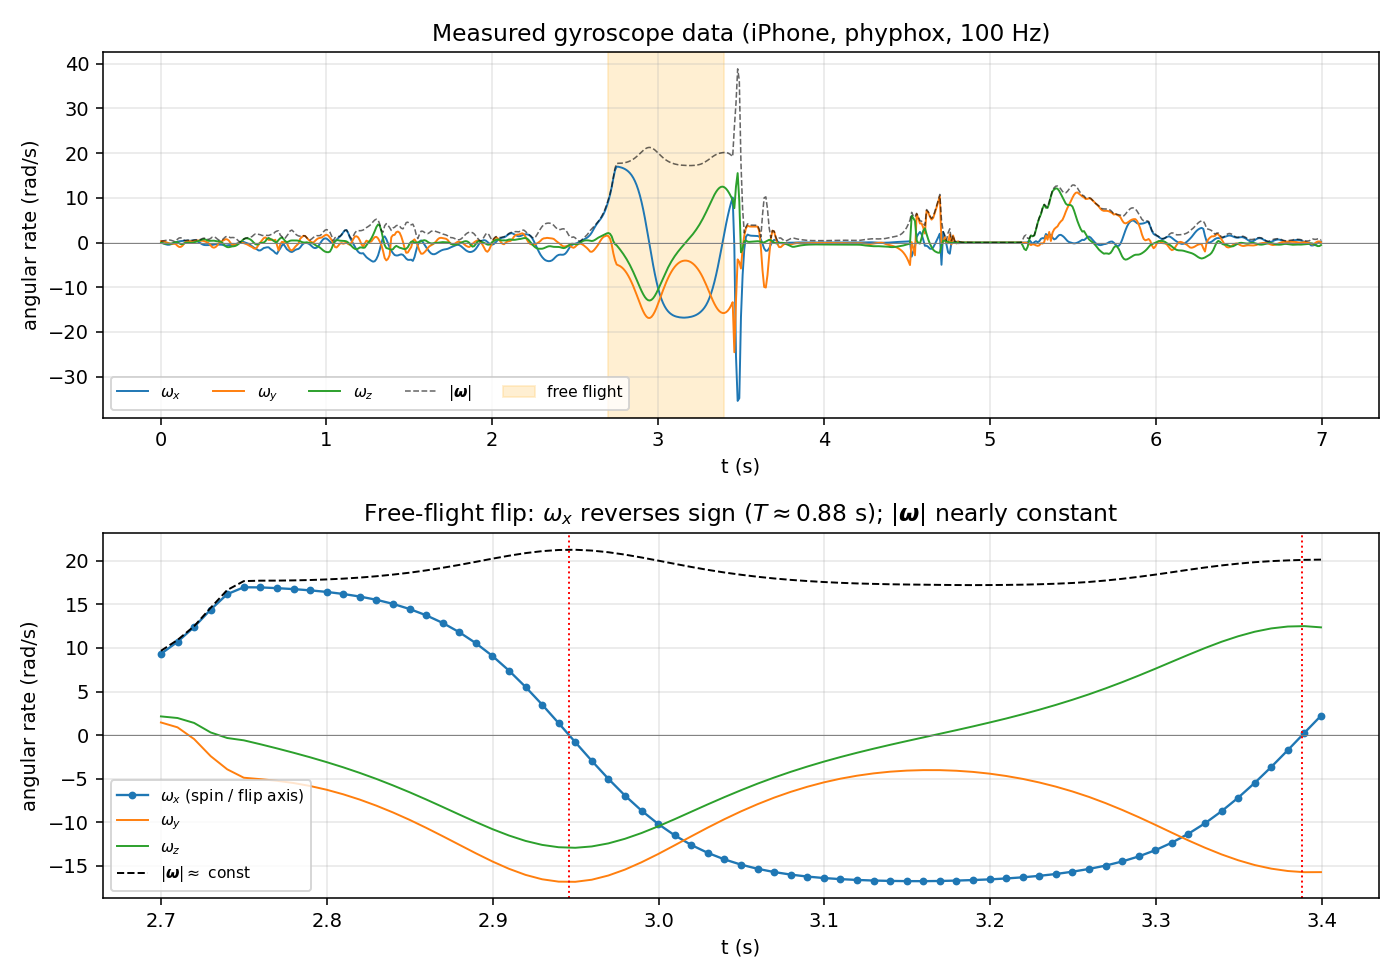
\includegraphics[width=0.92\linewidth]{figures/experiment_gyro.png}
\caption{Measured gyroscope data. \textbf{Top:} the full $7~\mathrm{s}$
recording with the free-flight window shaded; the spike at
$t\approx 3.5~\mathrm{s}$ is the catch. \textbf{Bottom:} zoom of the free
flight---$\omega_x$ reverses sign (red dotted zero crossings,
$T\approx 0.88~\mathrm{s}$) while $|\boldsymbol{\omega}|$ stays nearly constant.}
\label{fig:experiment}
\end{figure}

\begin{physicsinsight}
\textbf{Theory meets measurement.} The experiment confirms all three qualitative
predictions with nothing more than a phone and a free app: (i)
$|\boldsymbol{\omega}|$ is conserved to $\sim 10\%$ during free flight, (ii) the
intermediate-axis component flips sign while the perpendicular components surge,
and (iii) the motion is periodic. The chief departures from the idealized model
are the slow drag-induced decay of $|\boldsymbol{\omega}|$ (compare the
$-0.048~\mathrm{N\,m}$ mean torque measured by \cite{bubbar2025}) and the small
number of flip cycles captured in one short toss, which makes $T_{\text{flip}}$ an
estimate rather than a precise fit.
\end{physicsinsight}

% =========================================================================
\section{Critical Analysis and Commentary}
% =========================================================================
\begin{itemize}
\item \textbf{Implicit assumptions.} The conservative model neglects air drag,
which \cite{bubbar2025} showed is measurable (a slow $|\mathbf{L}|$ decay). It
also assumes a perfectly rigid body and exactly diagonal inertia tensor; real
objects flex and have product-of-inertia terms that we ignore.
\item \textbf{Degeneracy near $I_1 \approx I_2$.} The measured racquet sits
close to the symmetric-top limit, where our growth rate \eqref{eq:growth} is
small; the threshold between ``asymmetric'' and ``effectively symmetric''
behaviour is subtle and was left open in \cite{bubbar2025}.
\item \textbf{Pedagogical effectiveness.} The geometric sphere-ellipsoid
argument is visually compelling but hides the algebra; the linearisation in
Section~\ref{sec:derivations} is less elegant but makes the sign change
unmistakable. Presenting both, as we do here, is more convincing than either
alone.
\item \textbf{Extensions and applications.} The same instability governs the
tumbling of asteroids and the attitude control of spacecraft, where an
unintended intermediate-axis spin has wrecked real satellites~\cite{muller2019}.
A natural extension is to add a small damping torque and watch the body migrate
toward rotation about its axis of \emph{maximum} inertia (the minimum-energy
state at fixed $|\mathbf{L}|$).
\end{itemize}

% =========================================================================
\section{Conclusion}
% =========================================================================
We unpacked the intermediate axis theorem from first principles. Beginning with
the torque-free Euler equations~\eqref{eq:euler}, we derived the energy and
angular-momentum invariants and performed an explicit linear stability analysis
showing that the characteristic coefficient changes sign only for the
intermediate axis, yielding the exponential growth rate~\eqref{eq:growth}. A
custom RK4-plus-quaternion simulation then confirmed every prediction: it
reproduced the periodic $180^\circ$ flip, conserved $E$ and $|\mathbf{L}|$ to
$\sim 10^{-13}$, displayed the separatrix polhode geometry, and recovered the
inverse period--speed law of Bubbar \& Zhu. Working through the intermediate
mathematical steps---rather than accepting ``it can be shown''---turned a
baffling party trick into a transparent consequence of nonlinear coupling in
rigid-body dynamics.

% =========================================================================
\begin{thebibliography}{99}
% =========================================================================
\bibitem{bubbar2025}
Bubbar, F., \& Zhu, L. (2025).
\textit{The Intermediate Axis Theorem: A Model for the Period and a Phenomenal
Explanation.} Science One Programme, University of British Columbia.
\bibitem{peterson2021}
Peterson, C., \& Schwalm, W. (2021).
``Euler's rigid rotators, Jacobi elliptic functions, and the Dzhanibekov or
tennis racket effect.'' \textit{American Journal of Physics}, \textbf{89}(4),
349--357.
\bibitem{landau1976}
Landau, L. D., \& Lifshitz, E. M. (1976).
\textit{Mechanics} (3rd ed.). Butterworth--Heinemann.
\bibitem{goldstein2002}
Goldstein, H., Poole, C. P., \& Safko, J. L. (2002).
\textit{Classical Mechanics} (3rd ed.). Addison--Wesley.
\bibitem{ashbaugh1991}
Ashbaugh, M. S., Chicone, C. C., \& Cushman, R. H. (1991).
``The twisting tennis racket.'' \textit{Journal of Dynamics and Differential
Equations}, \textbf{3}(1), 67--85.
\bibitem{parker2020}
Parker, M., \& Hunt, H. (2020).
``Ellipsoids and the bizarre behaviour of rotating bodies.'' (Online lecture).
\bibitem{muller2019}
Muller, D. (2019).
``The Bizarre Behavior of Rotating Bodies.'' \textit{Veritasium} (online video).
\bibitem{phyphox}
Staacks, S., H\"utz, S., Heinke, H., \& Stampfer, C. (2018).
``Advanced tools for smartphone-based experiments: phyphox.''
\textit{Physics Education}, \textbf{53}(4), 045009.
\end{thebibliography}
\end{document}
